\section{Subject Environments - RQ1}\label{sec:environments}


 
%\claudio{Update the caption of the table to be a bit more specific}

%\deleted[id=CM]{Some environments were installed (I), others are web based (W) while in other we relied on documentation (D) either as a website, technical documentation or publications about the environments. For environments which are not web based and were not installed, compatibility of software and software policy were  the main reasons for not installing them.}

%\tb{Swaib, can you write a summary about the environments? (not much more than half a page); the original text is commented out below in the Latex file}
%\tb{is there a difference between block-based and blockly-based?} \swaib{blockly-based is an instance of block-based. Block-based means use of graph blocks/icons to represent programming concepts}



\begin{figure}[t]
     \centering
    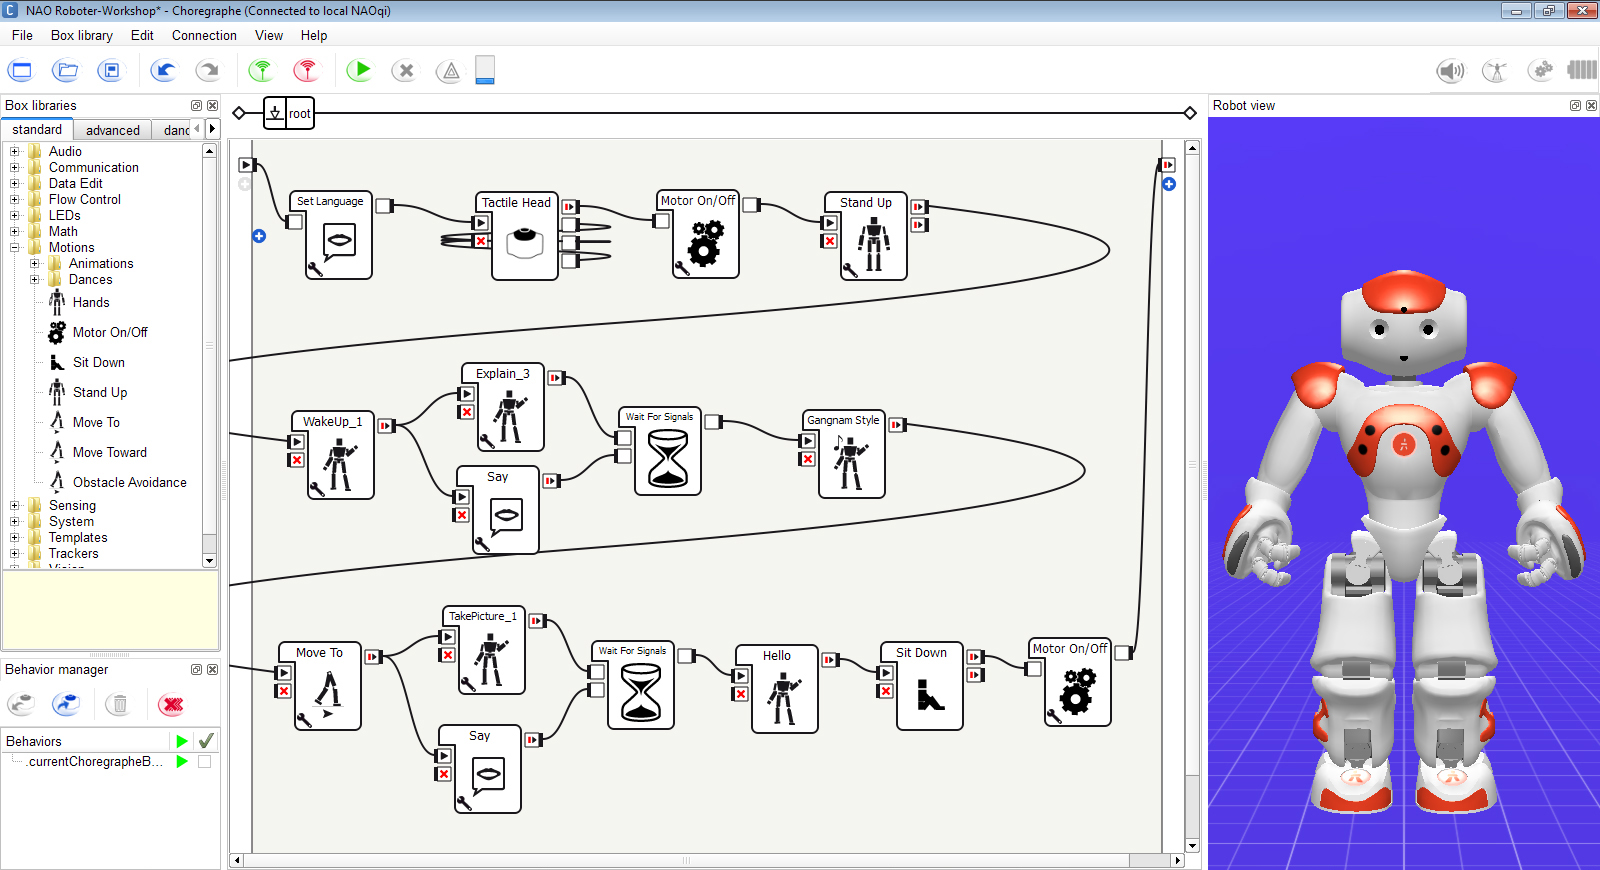
\includegraphics[width=\columnwidth]{fig/examples/choregraphe.jpg}
      \caption{The environment \choregraphe for the robot NAO}
      \label{fig:choregraphe}
   \end{figure}

In the following we provide a high-level textual description of the  subject environments identified (the interested reader might find the complete list of environments in Appendix).\\
%\begin{comment}
\parhead{\picaxe} (specifically, Blockly for Picaxe) is a programming environment for PICAXE chip-based robots such as the PICAXE 20X2 microbot. The \picaxe editor (PE) provides textual (in a Basic-style language) and Flowchart-based interface.  %\deleted[id=CM]{, as well as the tool Blockly for \picaxe, relying on the Blockly library realizing the visual syntax}.

%The current version PE6 provides graphical programming using either Blockly or Flow chart while text programming is done using Basic with simulation support~\cite{PICAXE}.% The environment has code generation wizards like pwmout and tune to generate code from the graphical notations.
%Logicator Flowcharting software is one of the programming techniques used in \picaxe in which flowcharting cells are used build a robot program. Such cells include: start, stop, process, and input.
%http://www.picaxe.com/Teaching/Logicator-Flowcharting-Software


\parhead{\ardublockly} is a Blockly-based graphical environment that generates python code for Arduino boards. The environment is used for programming Spartan robot ~\cite{Spartan}.% and can run on windows, Mac OS X, and Linux operating systems. The editor supports programming based on dragging and dropping of blocks, with code block warning and the code is compatible with variety of Arduino board based . 

\parhead{\openroberta} is a web-based environment for programming a variety of robots. It can either be run on the cloud  or installed on a local server. The  robots that can be programmed in Open Roberta include: Lego Mindstorms EV3, NXT, Calliope mini, micro:bit, Bot' n Roll[beta], Nao [beta], BOB3 [beta] ~\cite{OpenRoberta,Jost2015,Ketterl2015}. %The environment supports code generation in python, java, javascript and C/C++ depending on the particular robot being programmed. The graphical interface implements blockly code blocks for programming the robots. 

\parhead{\arcbotics} provides blockly-based  programming environment for Sparki robot, which generates C/C++ code for the robot to execute~\cite{ArcboticSparki}. %The colourful blocks help in syntactic support during programming to guide right order of assembling the blocks. 

\parhead{\edison} is an environment that provides Edblocks and Edscratch graphical notation while Edpy for textual notation. The current versions of Edison robots supported are V1 and V2 ~\cite{Edison}.%As Edblock provides programming blocks in which programmer provides parameters of a block, Edscratch provides symbolic block which depicts what the block actually does. This makes Edscratch more closer to the user domain. The graphical notations generate code in python 

\parhead{\missionlab} is an environment in which missions are specified through a state machine based graphical language. Missions can be executed on a simulator or on the robots ATRV-Jr, Urban Robot, AmigoBot, Pioneer AT, and Nomad 150 \& 200  ~\cite{arkin2002missionlab,Ulam2007}.%. During specification, each robot is generated its own state machine to execute. The current version V7 was released in 2006 and run on Red Hat linux, Fedora, Ubuntu, OpenSuse, Debian and CentOS 

\parhead{\flyaq} is a mission specification environment that allows specifying a mission by relying on an actual map of the environment in which the mission has to be executed. It allows users to specify  flight locations, no-fly zones for drones;  based on these information it automatically generates the flight plan for execution ~\cite{FLYAQ,DiRuscio2014,Bozhinoski2016}.%The environment runs in a virtual environment tailored to support the drone specific drivers needed to execute the missions. FLYAQ is a stack of language ranging from Monitoring mission language which provides interface to user; to behavioral language and the robot language  As an open source environment, extensions can be done to support more variety of robots. 

\parhead{\tivipe} is a visual programming environment that provides graphical notation for end-users to program NAO humanoid robot. The code blocks are abstracted into graphical modules making it a suitable end-users\,\cite{TiViPE}.  %"The aim is to let end-users develop software programs in a specific domain, without the need to have experience with textual programming languages" . Active users are psychologists for training children diagnosed with autism using NAO humanoid robot~\cite{Lourens2011}.
\tb{from a paper: ``The TiViPE concept of visual programming is to wrap
a routine that is constructed in a textual programming language
into a graphically represented unit. The main reason
for this concept is that there are many software libraries
available, but due to lack of documentation and a clear
structure most of these libraries remain unused. By making
all routine calls available as graphical units together with
appropriate documentation these routines can be made accessible
through TiViPE''\,\cite{lourens:2004:tivipe}}

\parhead{\aseba} is a collection of graphical and text based tools for programming thymio robots. The visual programming tool provides icons of events and corresponding actions to build a program ~\cite{ASEBA,Magnenat2011}. %The block based version uses blockly to provide program modules in which users edit the program variables to build an executable program. Its text based programming is done using Aseba language. The studio can be installed on Linux, Mac and Windows computers  .

\parhead{\sphero} is an environment used for programming Sphero BOLT, SPRK+, and Sphero Mini robots~\cite{Sphero}. %The application can be installed in iPads, android phones, iOS, Chrome machines, Mac and Windows systems. The graphical interface uses scratch blocks while text based programming is done using Java script. 

\parhead{\vex} provides an environment for programming VEX based robots like VEX EDR V5 and VEX IQ. 
%The studio runs on Mac and windows computer with graphical notation using ModKitBlock; a scratch based editor. 
The textual editing variances include ModkitText with high level of abstraction to C/C++~\cite{VexCodingStudio}.
%Pro which takes to general purpose programming environment with minimum levels of abstraction on robot related concepts
 %The studio takes care of all levels expertise in programming ranging from novices to experts. 

\parhead{\robotmesh} provides an environment for programming VEX robots~\cite{RobotMeshStudio}. 
%Unique in the stack of programming options is Flowol, a flow chart based graphical interface for specifying robotic missions. %It also support block based programming using blockly and python based text programming. The studio can be run online, the offline version only runs on windows
%~\cite{RobotMeshStudio}.

\parhead{\trik} is a flow-chart-based programming environment in which blocks connected to the chart are symbols of functions the block does. The studio provides an interactive simulation mode and supports multiple robots types like quadrocopters Geoscan Pioneer, robots LEGO Mindsorms NXT 2.0, and EV3~\cite{STRIKStudio, Mordvinov2017}. 

\parhead{\makeblock} supports programming micro:bit and makeblock robots using Scratch 3.0~\cite{Makeblock}. %Python is used for text based programming with abstractions for IoT and artificial intelligence
%~\cite{Makeblock}.

\parhead{\metabot} is a blockly based graphical programming environment that allows the definition of custom blocks and code generation logic for metabot v1 and v2 robots~\cite{Passault2016,Metabot}. %The environment generate assembly code for our custom virtual machine, which is then assembled to bytecode that can be simulated or run on actual robot. The virtual machine is cross-compiled with emscripten, and reads motor target angles to synchronize the 3D view
%~\cite{Passault2016,Metabot}. 
\Figref{metabot} shows a program demonstrating the use of loop control structure with a corresponding assembler code generated\,\cite{Metabot,Passault2016}. 

\begin{figure}[t]
     \centering
    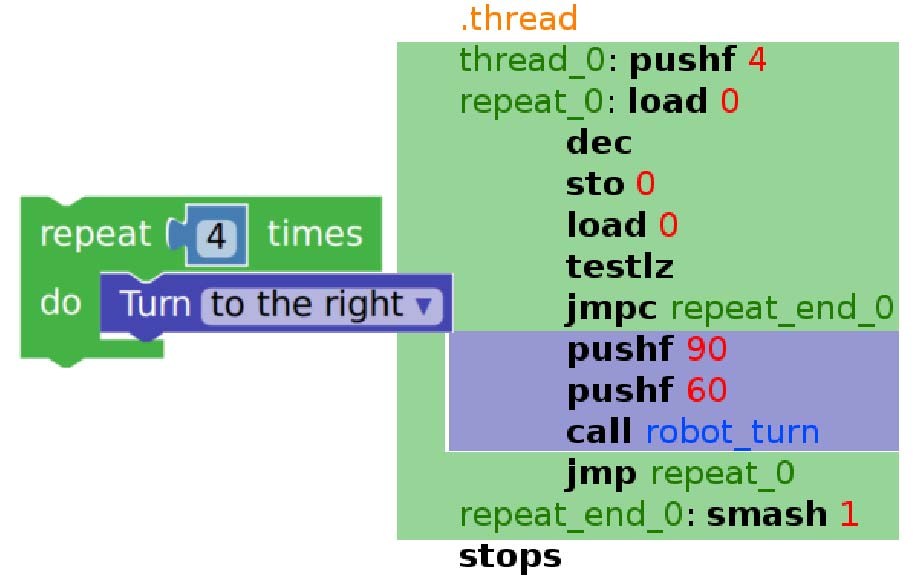
\includegraphics[width=.65\columnwidth]{metabotsample.jpg}
      \caption{Example of \metabot's visual notation (left), together with generated assembler code (right) for it (from\,\cite{Passault2016})}
      \label{metabot}
   \end{figure}



\parhead{\marty} is a Scratch-based environment for the marty robot. The environment has also customized python to martypy. It is a collection of code that abstracts key robot functions, making it high level for robotic programming as shown in \figref{scratch-marty}\,\cite{Marty}. 

\begin{figure}[t]
     \centering
    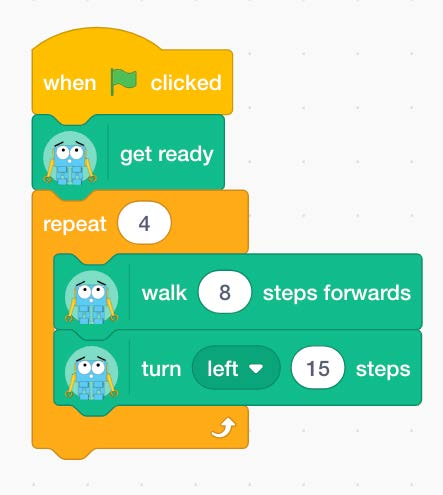
\includegraphics[width=.5\columnwidth]{ScratchMarty.jpg}
      \caption{Scratch for the robot Marty\,\cite{Marty} }
      \label{scratch-marty}
   \end{figure}

\parhead{\tello} is a Scratch-based application that generates code in Python for the drone Tello\,\cite{TelloEduApp}. %It provides assistance for the unique features, including the landmark maps for recognition and the skipping function between the landmark maps, and multi-machine flying formation\
 The environment is essentially Scratch extended with a library that imports Tello-specific blocks (mainly drone flight controls) into Scratch.

\parhead{\codelab}, like most educational environments, provides two variants of graphical programming: sandbox for novice programmers and constructor for advanced programmers using scratch blocks to program Cozmo robot~\cite{COZMO}.
%; What makes the constructor mode unique is the extra features like variables, functions and math operators\
  %The graphical application runs on android phones while text programming can be done on Mac, windows and Linux machines using python.

\parhead{\lego} is a programming environment equipped with tools and features to program Lego robots, and, among others also Ev3 and NXT~\cite{LEGO,alternativeLEGO}. %The robots can be programmed using computers, tablets or smart phones that can run Windows, Mac, iOS, Android, and iPad
 %It is block based graphical notation in which each block is an icon of the function it executes.  The lego robots can also be programmed in text using python, javascript, C/C++ though these are not part of the Lego mindstorms graphical environment.

\parhead{\choregraphe} is a multi-platform desktop application, allowing you to create animations, behaviors and dialogs, test them on a simulated robot or directly on a real one, and monitor and control your robot (NAO)~\cite{choregraphe,Monceaux2009,Miskam2014}, %The graphical interface provides a flow chart like interface in which programmer uses boxes, which are abstractions of mission concepts that are used to construct a behavior to be executed. The Python SDK can be used to directly program the NAO humanoid robot. Choregraphe's box libraries provide pre-program behaviors of the robot, work area for specifying missions and simulation window for the NAO robot
as shown in \figref{fig:choregraphe}.
%Choregraphe as a graphical environments supports robot control, behavior specification and access to sensor data for NAO robot ~\cite{Miskam2014}. 

\parhead{\blocklyprop} is a blockly based environment for specifying missions for ActivityBot robot\cite{Parallax}. %It is a web based environment with a client interface that can be used to connect the robot to the computer
%\,\cite{Parallax}.

\parhead{\ozoblockly} is a blockly-based visual programming environment\,\cite{ozobot} with five levels of complexity ranging from icon based blocks to advanced programming level, which offers low-level control functions and advanced programming features for programming ozobot.% https://ozoblockly.com/ last accessed 17th April 2019. 
 
\parhead{\minibloq} is a graphical environment for programming arduino robots like sparki, using icon based blocks~\cite{miniBloq}. %The environment is suited for kids from age four who are still learning to read/write and any person who has never been introduced to programming 
%~\cite{miniBloq}. %As an open source environment, more work is been done to accommodate advanced programmers.
  
\parhead{\turtlebot} enables novice programmers to quickly program the turtlebots~\cite{turtlebot3blockly}. %This is motivated by blockly's drag and drop feature, which has proved friendly in end-user programming
It provides a Blockly-based visual syntax and generates Python code for the turtlebot. %So far, Turtlebot3blockly supports two variants of turtlebot3, Waffle and Burger. 
 
\parhead{\makecode} provides a block-based visual editor and JavaScript based text editor for programming Lego Ev3 robot~\cite{makecode}. %JavaScript code is generated from the visual program, which can be downloaded to the computer to which the Lego robot is connected. Makecode is a platform managed by Microsoft to provide learning environment for programming. The environment provides a simulator for the supported robots
 
\parhead{\scratchev} is a customized version\,\cite{scratchEv3} of Scratch that allows the specification of missions for  Lego Mindstorms Eve3, WeDo, and Micro:bit robots. %As a web-based environment, you are expected to connect the robot to the computer to download and transfer the program to the robot for execution.

\parhead{\enchanting} is a  Scratch-based environment for programming Lego Mindstorm NXT robot by children~\cite{enchanting}. % The latest version was released in 2014
%\,\cite{enchanting}.% Enchanting allows the programmer to focus more on the end-user domain model, as its rich visual environment enables the user easily specify the mission for NXT robot.

\parhead{\easyc} is a graphical mission specification environment that provides a wizard-like interface with drag-drop support for specifying missions for VEX robots~\cite{EasyC}. %.  The programs are built as flow chart themes in which building blocks are icons of functional units of the program
%\,\cite{EasyC}. %It is tailored for students and teachers with basic programming skills, though it still provides organic C for advanced programmers.
%http://www.intelitek.com/engineering/easyc/ last accessed on 18th April 2019.


\parhead{\robotc} provides an environment that mixes graphical and textual elements, the RobotC natural language, to program robots\cite{robotc}.

%an easy ascent from graphical to text programming  by starting with a RobotC graphical, which provides a mix of graphical blocks with natural language expressions for beginners%. For those with familiarity with programming environments, yet not ready for syntax details of C language, can use RobotC natural language, where expression are in natural language, though using text. For advanced C programmers, RobotC gives high level of abstraction for robot controllers to ease programming experience, yet providing opportunity for creating new controllers
%\,\cite{robotc}.
%http://help.robotc.net/WebHelpMindstorms/index.htm  last accessed on 18th April 2019.
%\end{comment}